Considérons la fonction homographique $f$ définie sur $\intervalC{0}{\frac{\beta}{\alpha}}$ par $f(x) = \frac{- \alpha x + \beta}{x + \delta}$ où l'on suppose $(\alpha ; \beta ; \delta) \in (\RRsp)^3$ en utilisant des paramètres positifs comme en Physique.%
\footnote{
	Ces contraintes permettent d'obtenir la situation graphique proposée juste après.
}
%
Considérons $M$ un point sur $\setgeo*{C}{f}: y = f(x)$, et le rectangle $MNOP$ comme ci-dessous. Est-il possible de placer $M$ tel que $\area(MNOP)$ soit maximale?

\smallskip

\begin{center}
	\includegraphics[scale=.67]{goal.png}
\end{center}


% ----------------------- %


Pour minimiser le nombre de paramètres utilisés,
commençons par appliquer une dilatation horizontale de coefficient $\frac{\alpha}{\beta}$,
ce qui donne 
$g(x) = f( \frac{\beta}{\alpha} x ) 
      = \frac{\beta(1 - x)}{\delta + \frac{\beta}{\alpha} x}
      = \alpha \cdot \frac{1 - x}{\mu + x}$
en notant $\mu = \frac{\alpha \delta}{\beta}$.
Par confort,
appliquons ensuite une dilatation verticale de coefficient $\frac{1}{\alpha} > 0$,
ce qui fournit 
$h(x) = \frac{1 - x}{\mu + x}$.
%
Nous arrivons au problème de maximisation de
$\setgeo{A}(x) = x h(x) = \frac{x - x^2}{x + \mu}$
sur $\intervalC{0}{1}$.

\begin{stepcalc}[style=sar]
	\sder{\setgeo{A}}{1}(x)
\explnext{}
	\dfrac{(1 - 2 x)(x + \mu) - (x - x^2)}{(x + \mu)^2}
\explnext{}
	\dfrac{- x^2 - 2 \mu x + \mu}{(x + \mu)^2}
\end{stepcalc}

\smallskip

Nous sommes amener à étudier le signe du trinôme
$T(x) = - x^2 - 2 \mu x + \mu$.

\smallskip
\begin{stepcalc}[style=sar]
	\Delta
\explnext{}
	4 \mu^2 + 4 \mu
\explnext{}
	4 \mu (\mu + 1)
\end{stepcalc}
\smallskip

Comme $\mu > 0$, nous avons deux racines
$r_1 = - \mu - \sqrt{\mu (\mu + 1)}$
et
$r_2 = - \mu + \sqrt{\mu (\mu + 1)}$.
Or,
$0 < \mu < \mu + 1$
donne
$0 < r_2 < 1$,
puis
le tableau de variations suivant.
%
\begin{center}
	\begin{tikzpicture}
                \tkzTabInit[espcl=2.5]{
                	$x$                       / 1    ,
    				$T(x)$                    / 1.25 ,
    				$\sder{\setgeo{A}}{1}(x)$ / 1    ,
    				$\setgeo{A}(x)$           / 1.5
    			}{$0$, $r_2$, $1$}
    
                \tkzTabLine{ t , + , z , - , }
                \tkzTabLine{ t , + , z , - , }

                \tkzTabVar{-/ , +/, -/ }
	\end{tikzpicture}
\end{center}


Finalement,
$\area(MNOP)$ est maximale uniquement lorsque 
$x_M = \frac{\beta}{\alpha} r_2$,
c'est-à-dire pour % \mu = \frac{\alpha \delta}{\beta}
$x_M = \sqrt{\delta (\delta + \frac{\beta}{\alpha})} - \delta$
en revenant aux données initiales, car $\frac{\beta}{\alpha} \mu = \delta$.


% ----------------------- %


\begin{remark}
	Les calculs suivants montrent la concavité de $\setgeo{A}$, et donc de l'aire du rectangle initialement étudié.

	\smallskip
	\begin{stepcalc}[style=sar]
    	\sder{\setgeo{A}}{2}(x)
    \explnext{}
    	\dfrac{-2(x + \mu) \cdot (x + \mu)^2 - (- x^2 - 2 \mu x + \mu) \cdot 2(x + \mu) }{(x + \mu)^4}
    \explnext{}
    	\dfrac{- 2 x^2 - 4 \mu x - 2 \mu^2 + 2 x^2 + 4 \mu x - 2 \mu}{(x + \mu)^3}
    \explnext{}
    	\dfrac{- 2 \mu (\mu + 1)}{(x + \mu)^3}
    \end{stepcalc}
\end{remark}


% ----------------------- %


%\begin{remark}
%	XXX
%\end{remark}
